\chapter{Theory}

In this chapter, the theory behind technologies, on which this thesis is based on is described. It is all about wireless communication systems, which are indispensable nowadays. Most modern vehicles are already equipped with several wireless services for navigation (GNSS) and entertainment (Bluetooth, 4G etc.). In the future, vehicles will communicate among each other. \cite{V2XFuture}

\section{V2X-Communication}\label{sec:V2X-Communication}

Nowadays, most cars are equipped with security systems and sensors, which measure the environment. This data can be sent to other road users. The communication between a vehicle and anything surrounding it (Vehile2Anything or V2X) is grouped in vehicle to infrastructure (V2I), vehicle to vehicle (V2V) and vehicle to pedestrian (V2P). With V2X, vehicles can share information and data with other vehicles and objects in their surroundings. The goal is to warn other road users at an early stage to prevent traffic jams by redirecting their route. \cite{V2XFuture}

Data is transferred by wireless communication systems. There are two different standards, which are used for V2X communication. The Institute of Electrical and Electronics Engineers (IEEE) released the IEEE 802.11p-Standard. The 3rd Generation Partnership Project (3GPP) published the C-V2X standard. These are described in section \ref{ch:standarts}.

For vehicles, which communicate over V2X, an Onboard Unit (OBU) is built in. This device collects data of the car's position, speed, direction and the road conditions and sends them to other vehicles in its surroundings. \cite{Mustafa}

\section{GNSS}

A Global Navigation Satellite System (GNSS) is used to locate and navigate around the globe. A GNSS receiver can determine its position anywhere on earth. It is a broadcast system. Thus, the number of simultaneous users is unlimited. In addition to the position, those systems can determine the exact time, velocity and acceleration. A GNSS uses distance ranging for this information. A receiver can calculate the distance from different satellites by interpreting their signals. Additionally, it calculates the exact position of each satellite. Then its own position can be determined by computing the cross-section of the spheres around the satellites. \cite{WsCommScript}

Currently there are four active global navigation satellite systems in space. They differ mainly in frequency and modulation. The American GPS was the first system operating and therefore it is the most used. \cite{WsCommScript}

\newpage

\par
\underline{\large Systems and their provider:}\\

\begin{tabular}{ll}
	Global Positioning System (GPS) & America \\
	Global Navigation Satellite System (GLONASS) & Russia \\
	Galileo & European Union \\
	Beidou & China 
\end{tabular}

\section{Real Time Kinematic}

In some applications - as in this project - the position has to be determined accurately, for example to detect the right parking lot where the vehicle is situated. The GNSSs are not very accurate due to different weather conditions, inaccurate satellites clocks and bad constellations. To compensate these errors, a differential position detection is needed. With an additional base station, the listed errors can be determined and subtracted from the inaccurate position. With this method, the exact position of a moving object can be calculated as seen in figure \ref{fig:RTK}. It is called Real Time Kinematic (RTK) and can achieve an accuracy of a few millimeters, if the base station is less than 10\;km away from the vehicle. \cite{RTK} \cite{WsCommScript}

\begin{figure}[htb]
	\centering
	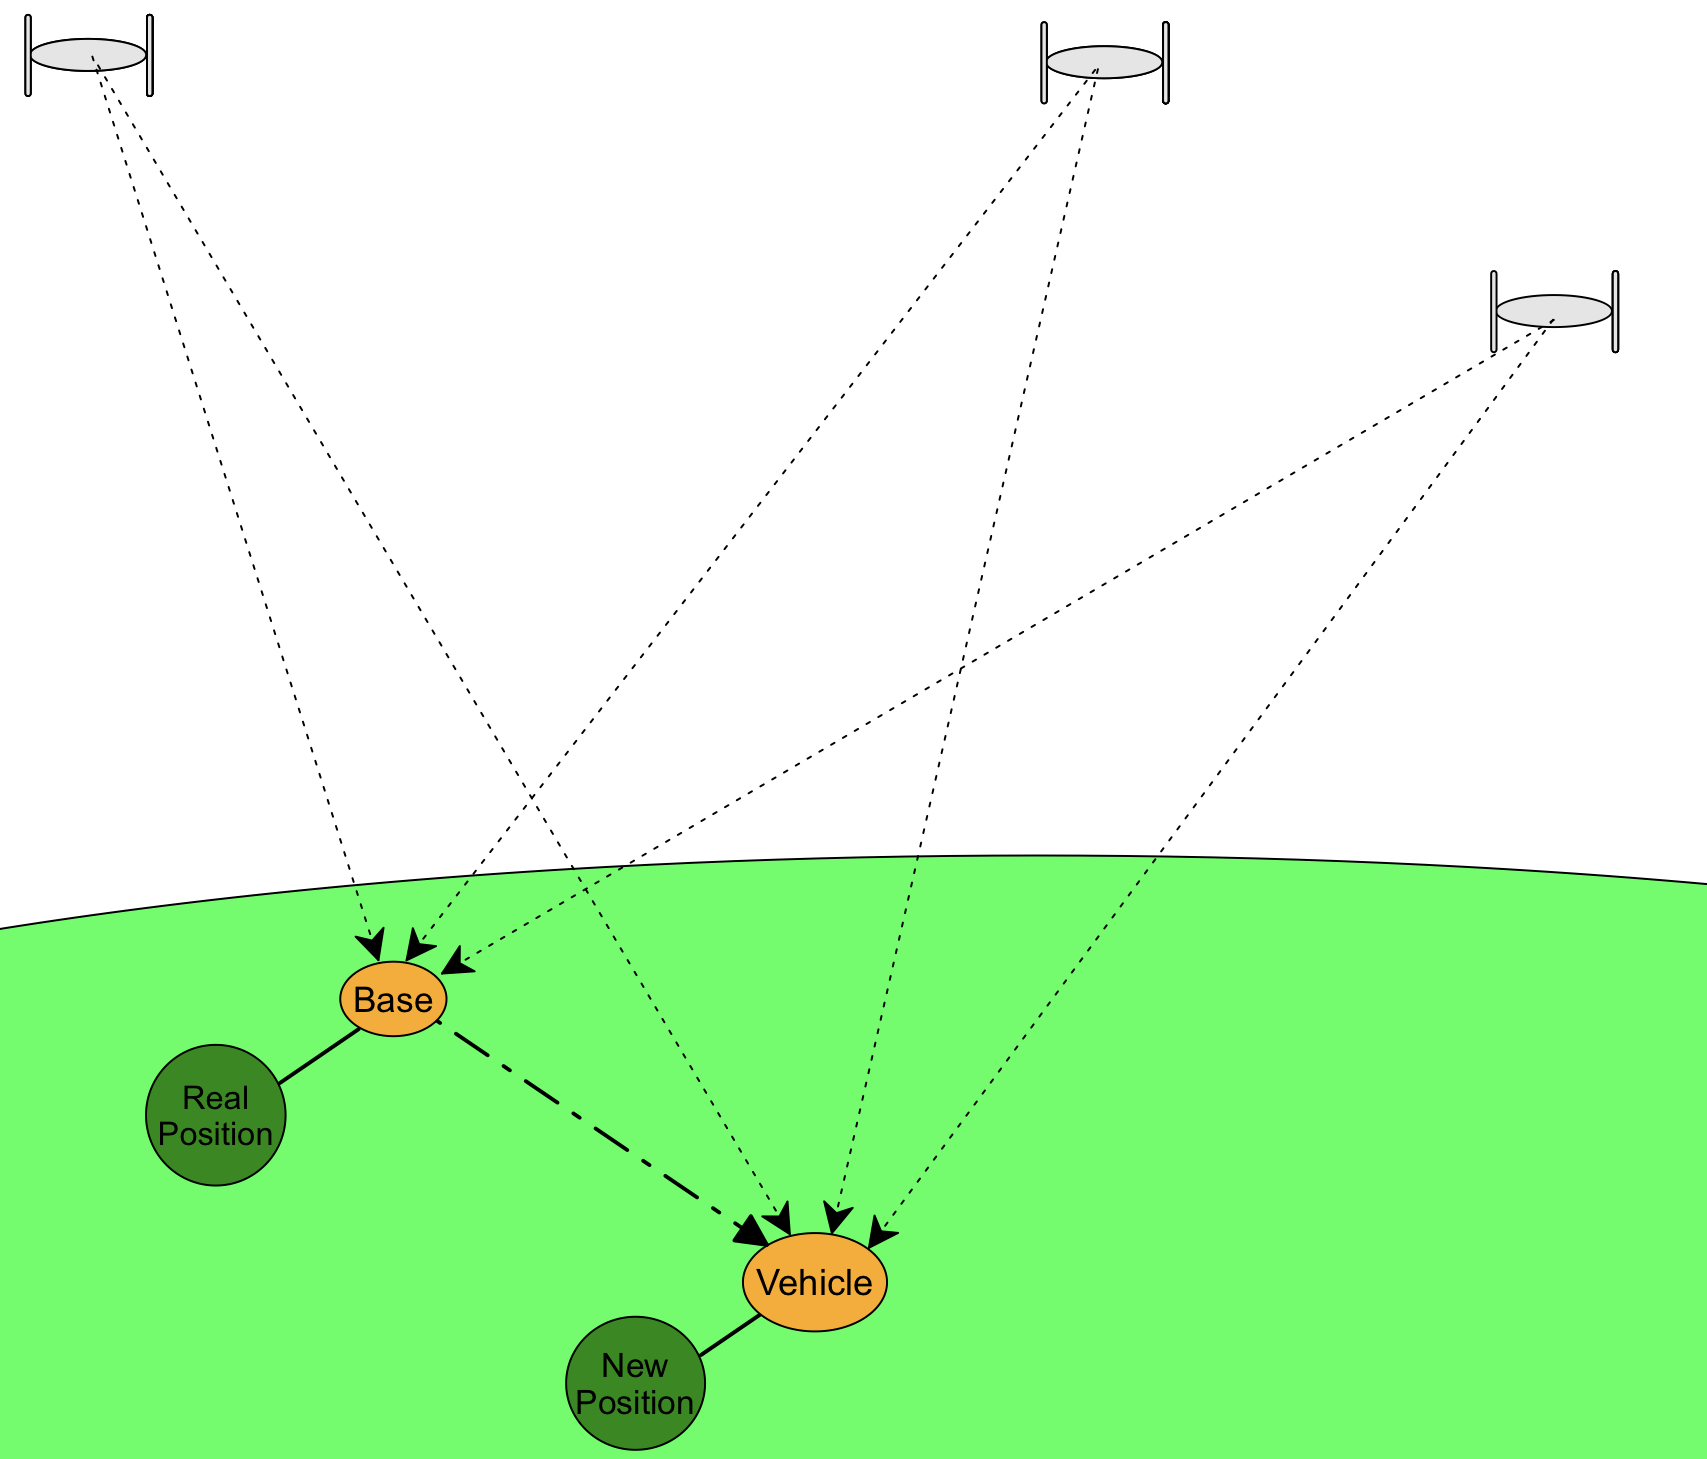
\includegraphics[width=0.8\textwidth]{images/RTK}
	\caption{Real Time Kinematic}
	\label{fig:RTK}
\end{figure}

\subsection{RTCM}

The Radio Technical Commission for Maritime Services (RTCM) is an international standards organization, which specifies radar systems, emergency position indication radio beacons, digital selective calling radios and differential GNSS. The latter of which is used in this thesis for the RTK application. More precisely the version RTCM 3 is used to send correction data to the Wireless Research Vehicle. \cite{RTCM}

\subsection{NTRIP}

The transmission of the data is done with Network Transport of RTCM via Internet Protocol (NTRIP). This is based on the Hypertext Transfer Protocol (HTTP). It is enhanced for GNSS data streams. The network can be built with different number of participants. Throughout this thesis, a single base station was enough, because the precise position only has to be known at the university campus. Additionally, there is only one rover - the wireless research vehicle. In this case, the RTCM messages can be transmitted directly from the NTRIP server to the client. The network can be extended for multiple participants. Which could be more vehicles or different applications with RTK. The correction data can be used in an area of a few kilometers around the university. The exact range depends on the accuracy. If future applications need RTK data at a greater distance, then more base stations have to be built in the specific area. In this case, a NTRIP caster is needed, which acts as a broadcaster between the servers and clients. It manages the handling of mountpoints for NTRIP sources. The whole network can be seen in the figure \ref{fig:NTRIP_model}. \cite{NTRIPApplication&Benefit} \cite{NTRIPV1}

\begin{figure}[htb]
	\centering
	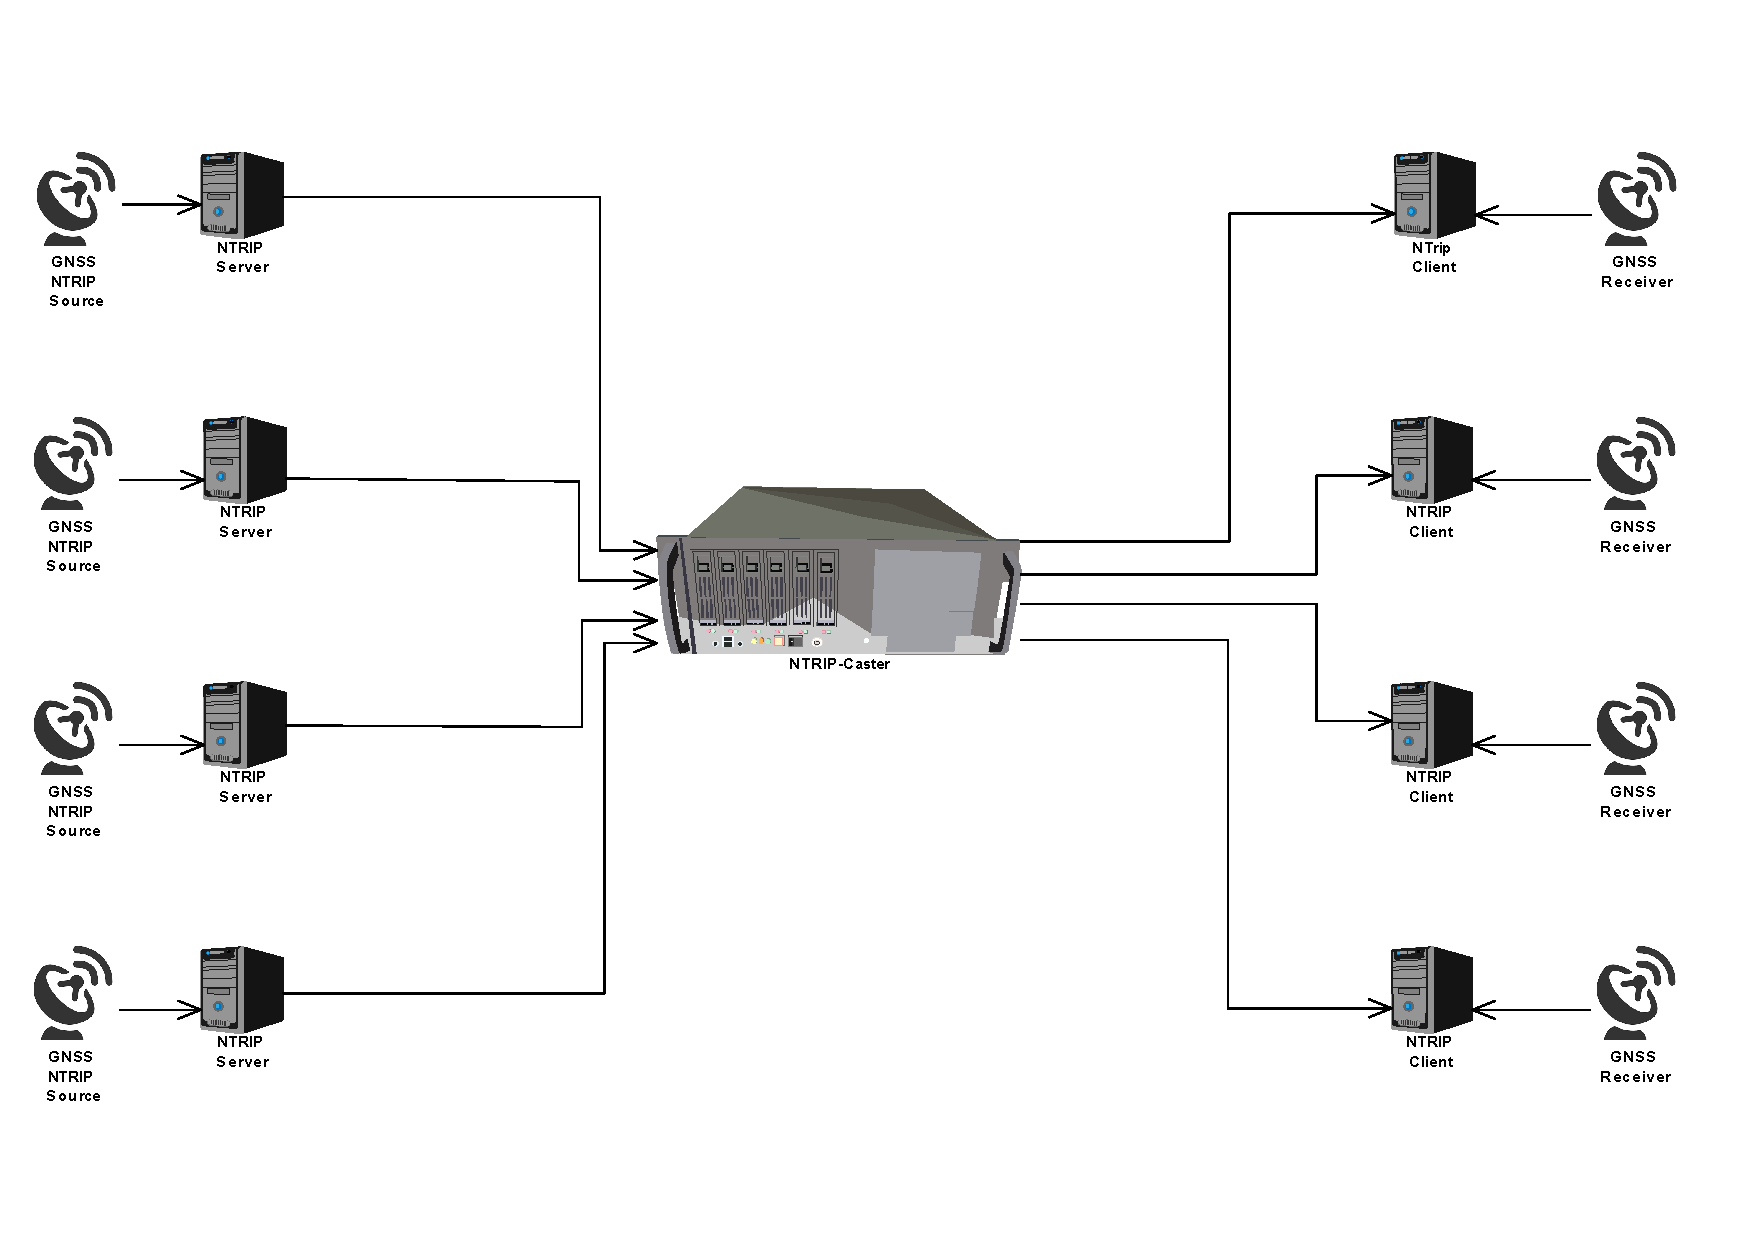
\includegraphics[width=0.8\textwidth]{images/NTRIP_model}
	\caption{NTRIP Network Model}
	\label{fig:NTRIP_model}
\end{figure}

\section{Authorization or Authentication}

Authentication is about verifying the identity of the user such as username, user ID and password. An authentication process ensures that the entities involved in an operation, are who they claim to be. This process is needed at charging stations as soon as the customer has to pay for the electricity. Then the system has to know, who to charge for this specific charging session.

Authorization occurs after the identification is successful. It verifies the rights of a user to allow access to resources in the system. For example, authorization can be used to check if the user is permitted to enter a garage or private parking area.
\cite{Auth}


\clearpage
\pagebreak